\documentclass[aspectratio=169]{beamer}

\usepackage{ccicons}
\usepackage{fontspec}
\usepackage{listings}
\usepackage{tikz}
\usepackage{svg}

\definecolor{uclablue}{RGB}{39,116,174}
\definecolor{uclagold}{RGB}{255,179,0}

\definecolor{ubcorange}{RGB}{158, 66, 37}

\definecolor{cugold}{RGB}{207, 184, 124}
\definecolor{cudarkgray}{RGB}{86, 90, 92}

\definecolor{solarizedred}{RGB}{220, 50, 47}
\definecolor{solarizedblue}{RGB}{38, 139, 210}
\definecolor{solarizedgreen}{RGB}{133, 153, 0}
\definecolor{solarizedpurple}{RGB}{108, 113, 196}
\definecolor{solarizedmagenta}{RGB}{211, 54, 130}

\definecolor{pantone655}{RGB}{0, 42, 92}
\definecolor{pantone7453}{RGB}{123, 164, 217}
\definecolor{pantone633}{RGB}{0, 139, 176}
\definecolor{pantone7492}{RGB}{218, 229, 205}

\colorlet{primarycolor}{pantone655}
\colorlet{secondarycolor}{pantone7453}


\usetikzlibrary{
  arrows,
  arrows.meta,
  automata,
  backgrounds,
  calc,
  chains,
  decorations.pathreplacing,
  fit,
  intersections,
  matrix,
  overlay-beamer-styles,
  positioning,
  shapes,
  shapes.multipart,
  tikzmark,
}
\usetikzmarklibrary{listings}

\hypersetup{
  colorlinks=true,
  urlcolor=cudarkgray,
}

\setbeamercolor{frametitle}{fg=primarycolor}
\setbeamercolor{structure}{fg=primarycolor}
\setbeamercolor{enumerate item}{fg=black}
\setbeamercolor{itemize item}{fg=black}
\setbeamercolor{itemize subitem}{fg=black}

\setbeamersize{text margin left=26.6mm}
\addtolength{\headsep}{2mm}

\setbeamertemplate{navigation symbols}{}
\setbeamertemplate{headline}{}
\setbeamertemplate{footline}{}
\setbeamertemplate{itemize item}{\color{black}}
\setbeamertemplate{itemize items}[circle]

\setbeamertemplate{footline}{
  \begin{tikzpicture}[remember picture,
                      overlay,
                      shift={(current page.south west)}]
    \node [black!50, inner sep=2mm, anchor=south east]
          at (current page.south east) {\footnotesize \insertframenumber};
  \end{tikzpicture}
}

\setsansfont{Inter}[Scale=MatchLowercase]
\setmonofont{Hack}[Scale=MatchLowercase]

\makeatletter
\newcommand\version[1]{\renewcommand\@version{#1}}
\newcommand\@version{}
\def\insertversion{\@version}

\newcommand\lecturenumber[1]{\renewcommand\@lecturenumber{#1}}
\newcommand\@lecturenumber{}
\def\insertlecturenumber{\@lecturenumber}
\makeatother

\setbeamertemplate{title page}
{
  \begin{tikzpicture}[remember picture,
                      overlay,
                      shift={(current page.south west)},
                      background rectangle/.style={fill=pantone655},
                      show background rectangle]
    \node [anchor=west, align=left, inner sep=0, text=white]
          (lecturenumber) at (\paperwidth / 6, \paperheight * 3 / 4)
          {\Large Lecture \insertlecturenumber};
    \node [inner sep=0, align=left, text=white, node distance=0,
          above left=of lecturenumber, anchor=south west, yshift=2mm]
          {\Large ECE 344: Operating Systems};
    \node (title) [inner sep=0, anchor=west, align=left, text=white,
                   text width=30em]
          at (\paperwidth / 6, \paperheight / 2)
          {{\bfseries \Huge \inserttitle{}}};
    \node [inner sep=0, align=right, text=white, node distance=0,
          below right=of title, anchor=north east, yshift=-1mm]
          {{\footnotesize \ttfamily \insertversion}};
    \node [inner sep=0, text=white, align=left, anchor=west]
          (author) at (\paperwidth / 6, \paperheight / 4)
          {\insertauthor};
    \node [text=white, inner sep=0, align=left, node distance=0,
           below left=of author, anchor=north west, yshift=-2mm]
          {\insertdate};
    \node [align=right, anchor=south east, inner sep=2mm, text=white]
          (license) at (\paperwidth, 0)
          {\footnotesize This  work is licensed under a
           \href{http://creativecommons.org/licenses/by-sa/4.0/}
                {\color{pantone7453} Creative Commons Attribution-ShareAlike 4.0
                 International License}};
    \node [text=white, inner sep=0, align=right, node distance=0,
           above right=of license, anchor=south east, xshift=-2mm]
          {\Large \ccbysa};
  \end{tikzpicture}
}

\tikzset{
  >=Straight Barb[],
  shorten >=1pt,
  initial text=,
}

\lstset{
  basicstyle=\footnotesize\ttfamily,
  language=C,
  escapechar=@,
  commentstyle=\color{black!50},
}


\lecturenumber{11}
\title{More Locks}
\version{1.0.0}
\author{Jon Eyolfson}
\date{October 3, 2022}

\begin{document}
  \begin{frame}[plain, noframenumbering]
    \titlepage
  \end{frame}

  \begin{frame}
    \frametitle{Locks Ensure Mutual Exclusion}

    Only one thread at a time can be between the \texttt{lock} and
    \texttt{unlock} calls

    \vspace{2em}

    It does not help you ensure ordering between threads
  \end{frame}

  \begin{frame}[fragile]
    \frametitle{Semaphores are Used for Signaling}

    Semaphores have a {\tt value} that's shared between threads/processes

    \vspace{2em}

    \begin{lstlisting}
#include <semaphore.h>

int sem_init(sem_t *sem, int pshared, unsigned int value)
    \end{lstlisting}

    \vspace{2em}

    There may up to \texttt{value} number of things with the semaphore
    simultaneously

    \vspace{2em}

    It has two fundamental operations {\tt wait} and {\tt post}

    \hspace{2em} \texttt{wait} decrements the value atomically

    \hspace{2em} \texttt{post} increments the value atomically

    \vspace{2em}

    If \texttt{wait} will not return until the value is greater than 0
  \end{frame}

  \begin{frame}[fragile]
    \frametitle{Semaphore API is Similar to \texttt{pthread} Locks}
  
    \begin{lstlisting}
#include <semaphore.h>

int sem_init(sem_t *sem, int pshared, unsigned int value)
int sem_destroy(sem_t *sem);
int sem_post(sem_t *sem);
int sem_wait(sem_t *sem);
int sem_trywait(sem_t *sem);
    \end{lstlisting}

    \vspace{2em}

    All functions return 0 on success

    \vspace{2em}

    The \texttt{pshared} argument is a boolean, you can set it to \texttt{1} for
    IPC

    \hspace{2em} For IPC the semaphore needs to be in shared memory
  \end{frame}

  \begin{frame}[fragile]
    \frametitle{How Could We Make This Print ``Thread 1'' then ``Thread 2''?}

    \begin{lstlisting}
#include <pthread.h>
#include <stdio.h>
#include <semaphore.h>
#include <stdlib.h>

void* p1 (void* arg) { printf("Thread 1\n"); return NULL; }

void* p2 (void* arg) { printf("Thread 2\n"); return NULL; }

int main(int argc, char *argv[])
{
    pthread_t thread[2];
    pthread_create(&thread[0], NULL, p1, NULL);
    pthread_create(&thread[1], NULL, p2, NULL);
    pthread_join(thread[0], NULL);
    pthread_join(thread[1], NULL);
    return EXIT_SUCCESS;
}
    \end{lstlisting}
  \end{frame}

  \begin{frame}[fragile]
    \frametitle{This Code Prints ``Thread 1'' then ``Thread 2''}

    \begin{lstlisting}[escapechar=!]
!\structure{static sem\_t sem;}!

void* p1 (void* arg) {
  printf("Thread 1\n");
  !\structure{sem\_post(\&sem);}!
}

void* p2 (void* arg) {
  !\structure{sem\_wait(\&sem);}!
  printf("Thread 2\n");
}

int main(int argc, char *argv[])
{
  !\structure{sem\_init(\&sem, 0, 0);}!
  /* rest as before */
}
    \end{lstlisting}
  \end{frame}

  \begin{frame}
    \frametitle{No Matter Which Thread Executes First, We Get the Same Order}

    The \texttt{value} is initially 0

    \vspace{2em}

    Assume ``Thread 2'' executes first

    \hspace{2em} It executes \texttt{sem\_wait}, which is 0, and doesn't
    continue

    \vspace{2em}

    ``Thread 1'' doesn't have to wait, it prints first before it increments the
    \texttt{value}

    \vspace{2em}

    ``Thread 2'' can then execute its print statement

    \vspace{2em}

    What happens if we initialized the \texttt{value} to 1?
  \end{frame}

  \begin{frame}
    \frametitle{We Can Use a Semaphore as a Mutex}

    How?
  \end{frame}

  \begin{frame}[fragile]
    \frametitle{Using a Semaphore as a Mutex, Note the \texttt{value}}

    \begin{lstlisting}[escapechar=!]
...
!\structure{static sem\_t sem;}!
static int counter = 0;

void* run(void* arg) {
    for (int i = 0; i < 100; ++i) {
        !\structure{sem\_wait(\&sem);}!
        ++counter;
        !\structure{sem\_post(\&sem);}!
    }
}

int main(int argc, char *argv[])
{
  !\structure{sem\_init(\&sem, 0, 1);}!
  // Create 8 threads
  // Join 8 threads
  printf("counter = %i\n", counter);
}
    \end{lstlisting}
  \end{frame}

  \begin{frame}
    \frametitle{Can We Come Up with a Solution for a Producer/Consumer Problem?}

    Assume you have a circular buffer:

    \vspace{2em}

    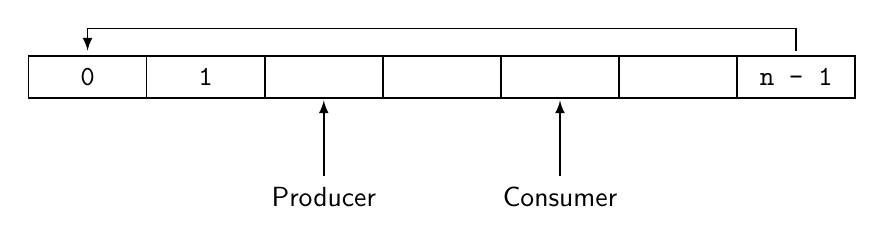
\begin{tikzpicture}[>=latex,font=\ttfamily,
      every node/.style={
        minimum width=1.5cm,
        minimum height=1.5em,
        outer sep=0pt,
        draw=black,
        semithick
      }
    ]
      \node at (0,0) (A) {0};
      \node [anchor=west] at (A.east) (B) {1};
      \node [anchor=west] at (B.east) (C) {};
      \node [anchor=west] at (C.east) (D) {};
      \node [anchor=west] at (D.east) (E) {};
      \node [anchor=west] at (E.east) (F) {};
      \node [anchor=west] at (F.east) (G) {n - 1};
      \draw [->,shorten >=2pt,shorten <=2pt,semithick] (G.north) -- +(0,1em) -| (A);

      \node [below=of C, draw=none] (producer) {\sffamily Producer};
      \draw [->, semithick] (producer) -- (C);

      \node [below=of E, draw=none] (consumer) {\sffamily Consumer};
      \draw [->, semithick] (consumer) -- (E);
    \end{tikzpicture}

    \vspace{2em}

    The producer should write to the buffer

    \hspace{2em} As long as the buffer is not full

    \vspace{2em}

    The consumer should read to the buffer

    \hspace{2em} As long as the buffer is not empty
  \end{frame}

  \begin{frame}[fragile]
    \frametitle{We Would Create Two Semaphores, What \texttt{value}s Should We Use?}

    \begin{lstlisting}
sem_t full;
sem_t empty;

sem_init(&full, 0, /* ??? */);
sem_init(&empty, 0, /* ??? */);

void producer() {
  // produce data
  sem_wait(empty);
  // fill a slot
  sem_post(full);
}

void consumer() {
  sem_wait(full);
  // empty a slot
  sem_post(empty);
  // consume data
}
    \end{lstlisting}
  \end{frame}

  \begin{frame}
    \frametitle{The Previous \texttt{value}s Depend on the Buffer Size}

    \texttt{full} should always be initialized to 0

    \vspace{2em}

    \texttt{empty} should be initialized to the size of the buffer ---
    \texttt{N}

    \vspace{2em}

    Do we need any extra locking?

    \onslide<2->{
      \hspace{2em} No, if there's a single producer and consumer

      \hspace{2em} Yes, otherwise
    }
  \end{frame}

  \begin{frame}
    \frametitle{Monitors Are Built Into Some Languages}

    With object oriented programming, developers wanted something easier to use

    \vspace{2em}

    Could mark a method as monitored, and let the compiler handle locking

    \hspace{2em} An object can only have one thread active in its monitored
    methods

    \vspace{2em}

    It's basically one mutex per object, created for you

    \hspace{2em} The compiler inserts calls to lock and unlock
  \end{frame}

  \begin{frame}[fragile]
    \frametitle{Java's \texttt{synchronized} Keyword is an Example of a Monitor}

    \begin{lstlisting}
public class Account {
  int balance;
  public synchronized void deposit(int amount)  { balance += amount; }
  public synchronized void withdraw(int amount) { balance -= amount; }
}
    \end{lstlisting}

    the compiler transforms to:

    \begin{lstlisting}[escapechar=!]
  public void deposit(int amount) {
    !\structure{lock(this.monitor);}!
    balance += amount;
    !\structure{unlock(this.monitor);}!
  }
  public void withdraw(int amount) {
    !\structure{lock(this.monitor);}!
    balance -= amount;
    !\structure{unlock(this.monitor);}!
  }
    \end{lstlisting}
  \end{frame}

  \begin{frame}[fragile]
    \frametitle{Condition Variables Behave Like Semaphores}

    You can create your own custom queue of threads

    \vspace{2em}

    \begin{lstlisting}
#include <pthread.h>

int pthread_cond_init(pthread_cond_t *cond,
                      const pthread_condattr_t *attr)
int pthread_cond_destroy(pthread_cond_t *cond);
int pthread_cond_signal(pthread_cond_t *cond);
int pthread_cond_broadcast(pthread_cond_t *cond);
int pthread_cond_wait(pthread_cond_t *cond, pthread_mutex_t *mutex);
int pthread_cond_timedwait(pthread_cond_t *cond, pthread_mutex_t *mutex,
                           const struct timespec *abstime);
    \end{lstlisting}

    \vspace{2em}

    The \texttt{wait} functions add this thread to the queue

    \hspace{2em} \texttt{signal} wakes up one thread, \texttt{broadcast} wakes
    up all threads
  \end{frame}

  \begin{frame}
    \frametitle{Condition Variables MUST Be Paired with a Mutex}

    Any calls to \texttt{wait}, \texttt{signal}, and \texttt{broadcast} must
    already hold the mutex

    \vspace{2em}

    Why? \texttt{wait} needs to add itself to the queue safely (without data
    races)

    \hspace{2em} It needs the mutex as an argument to unlock it before going to
    sleep

    \vspace{2em}

    One mutex can also protect multiple condition variables

    \vspace{2em}

    We'll only consider calls to \texttt{wait} and \texttt{signal}
  \end{frame}

  \begin{frame}[fragile]
    \frametitle{We Can Use Condition Variables for Our Producer/Consumer}

    \begin{columns}
      \begin{column}{0.5\textwidth}
        \begin{lstlisting}
pthread_mutex_t mutex;
int nfilled;
pthread_cond_t has_filled;
pthread_cond_t has_empty;

void producer() {
  // produce data
  pthread_mutex_lock(&mutex);
  if (nfilled == N) {
    pthread_cond_wait(&has_empty,
                      &mutex);
  }
  // fill a slot
  ++nfilled;
  pthread_cond_signal(&has_filled);
  pthread_mutex_unlock(&mutex);
}
        \end{lstlisting}
      \end{column}
      \begin{column}{0.5\textwidth}
        \begin{lstlisting}
void consumer() {
  pthread_mutex_lock(&mutex);
  if (nfilled == 0) {
    pthread_cond_wait(&has_filled,
                      &mutex);
  }
  // empty a slot
  --nfilled;
  pthread_cond_signal(&has_empty);
  pthread_mutex_unlock(&mutex);
  // consume data
}
        \end{lstlisting}
      \end{column}
    \end{columns}
  \end{frame}

  \begin{frame}
    \frametitle{Condition Variables Serve a Similar Purpose as Semaphores}

    You can think of semaphores as a special case of condition variables

    \hspace{2em} They'll go to sleep when the value is 0, when it's greater
    than 0 they wake up

    \vspace{2em}

    You can implement one using the other, however it can get messy

    \vspace{2em}

    For complex conditions condition variables offer much better clarity
  \end{frame}


  \begin{frame}
    \frametitle{We Explored More Advanced Locking}

    Before we did mutual exclusion, now we can ensure order

    \begin{itemize}
      \item Semaphores are an atomic value that can be used for signaling
      \item Condition variables are clearer for complex condition signaling
    \end{itemize}
  \end{frame}
\end{document}
